% Working draft for a JATIS-style instrumentation manuscript.
% TODO: replace this generic article preamble with the official SPIE/JATIS
% journal template before submission.
\documentclass[10pt,letterpaper]{article}

\usepackage[margin=1in]{geometry}
\usepackage{graphicx}
\usepackage{amsmath,amssymb}
\usepackage{booktabs}
\usepackage{siunitx}
\usepackage{xcolor}
\usepackage{hyperref}
\usepackage{caption}
\usepackage{subcaption}
\usepackage{enumitem}
\usepackage{microtype}
\usepackage[backend=biber,style=numeric,sorting=none,maxbibnames=8]{biblatex}
\addbibresource{references.bib}

\graphicspath{{figures/}}
\hypersetup{
  colorlinks=true,
  linkcolor=blue!50!black,
  citecolor=blue!50!black,
  urlcolor=blue!50!black
}

\sisetup{detect-all=true,per-mode=symbol}

\newcommand{\pfa}{P_{\mathrm{FA}}}
\newcommand{\pd}{P_{D}}
\newcommand{\fstat}{T}
\newcommand{\todo}[1]{\textcolor{red!70!black}{\textbf{[TODO: #1]}}}
\newcommand{\paperone}{\texttt{paper1\_small}}

\title{A calibrated pilot-tone F-statistic detector and GPU prototype for digital-television RFI mitigation in radio astronomy}

\author{\begin{tabular}{c}
Dylan J. Gormley$^{1,2}$ and Kevin M. Bandura\\[1mm]
\small $^{1}$Lane Department of Computer Science and Electrical Engineering, West Virginia University, Morgantown, WV, USA\\
\small $^{2}$Center for Gravitational Waves and Cosmology, West Virginia University, Morgantown, WV, USA\\[1mm]
\small \texttt{dylan.gormley@mail.wvu.edu}
\end{tabular}}

\date{Draft: \today}

\begin{document}
\maketitle

\begin{center}

\end{center}

\begin{abstract}
Digital television (DTV) transmissions are a persistent source of structured radio-frequency interference (RFI) in the 400--800 MHz band used by several radio astronomy experiments. Unlike impulsive or transient RFI, ATSC 1.0 broadcasts can remain continuously present while varying in received strength, making simple power thresholding or schedule-based avoidance incomplete. We present a pilot-tone detector that exploits the narrow ATSC 1.0 pilot located near the lower edge of each 6 MHz broadcast channel. The detector forms a local F-statistic from target bins around the pilot and reference bins separated by guard bins. For the current implementation, the detector uses $K=128$ fine bins, $M=1{,}048{,}576$ accumulated samples, four guard bins, and an analytic null model with $df_1=2{,}097{,}152$ and $df_2=4{,}194{,}304$. We validate the null distribution with 300,000 Monte Carlo trials, calibrate constant-false-alarm-rate thresholds, characterize detection probability as a function of DTV data-shelf SNR, and quantify robustness to within-bin offsets, Doppler offsets, gain/noise perturbations, and reference-bin leakage. We also describe a fixed-point CUDA prototype and benchmark its current kernel-only throughput. Finally, we demonstrate the detector on a short recorded DTV-contaminated segment, producing pilot-level and expanded DTV masks. The current real-data example is a single-segment demonstration rather than archive-scale validation; long-duration tests and science-driven threshold selection are deferred to future work.
\end{abstract}

\noindent\textbf{Keywords:} radio-frequency interference; radio astronomy instrumentation; digital television; ATSC 1.0; constant false alarm rate; GPU implementation; 21 cm intensity mapping

\section{Introduction}

Radio-frequency interference (RFI) is a central design constraint for modern radio astronomy. It affects single-dish observations, interferometric imaging, fast-transient searches, pulsar observations, and 21 cm intensity mapping. Classical mitigation methods include power thresholding, statistical tests such as spectral kurtosis, morphological flag growth, spatial filtering, and post-processing flaggers such as AOFlagger \cite{FridmanBaan2001,Nita2007,NitaGary2010,Offringa2012,Mesarcik2022}. These methods are broadly useful but are not always matched to a specific engineered waveform. Persistent digital television (DTV) interference is a useful example: it is structured, occupies known broadcast channels, and can be continuously present.

This work focuses on ATSC 1.0 DTV interference in the radio astronomy band relevant to experiments such as CHIME, which observes across 400--800 MHz for 21 cm intensity mapping and transient science \cite{CHIMEOverview2022}. In North America, ATSC 1.0 channels have a 6 MHz structure and include a pilot near the lower edge of the channel. The ATSC A/53 standard describes a small pilot at the suppressed-carrier frequency, nominally about 309 kHz from the lower band edge \cite{ATSC_A53_Part2_2011}. The pilot is narrow compared with the data shelf, and therefore provides a known feature that can be exploited for detection.

The goal of this paper is to define, calibrate, and prototype a pilot-tone detector for DTV RFI masking. The detector is not meant to replace all RFI mitigation, and it is not a final telescope deployment report. Instead, it provides a statistically calibrated detection axis that can be used to generate DTV masks and can later be connected to downstream science tolerance. In particular, for 21 cm baryon acoustic oscillation (BAO) measurements, the final operating point should ultimately be selected from a science-loss budget rather than detector convenience alone. Fisher-forecast machinery such as RadioFisher provides a natural route for that later mapping \cite{Bull2015,RadioFisher2021}.

The paper is organized as follows. Section~\ref{sec:dtv_context} introduces the DTV pilot structure and recorded data used for the demonstration. Section~\ref{sec:detector} defines the F-statistic detector. Section~\ref{sec:calibration} validates the null model and sensitivity. Section~\ref{sec:robustness} characterizes robustness. Section~\ref{sec:implementation} describes the fixed-point GPU prototype. Section~\ref{sec:realdata} presents the single-segment recorded-data demonstration. Section~\ref{sec:discussion} discusses limitations and future work.

\section{DTV pilot context and data stream convention}
\label{sec:dtv_context}

Figure~\ref{fig:context} shows the motivating DTV-contaminated segment and the ATSC pilot/data-shelf structure. The recorded waterfall contains persistent horizontal structure at the DTV channel locations. The schematic panel shows the relevant 6 MHz channel scale, the pilot near the lower channel edge, and the broader data shelf. The detector developed here uses the pilot as a narrowband feature to infer when a DTV channel is active, then expands that pilot-level decision into a DTV mask.

\begin{figure}[t]
  \centering
  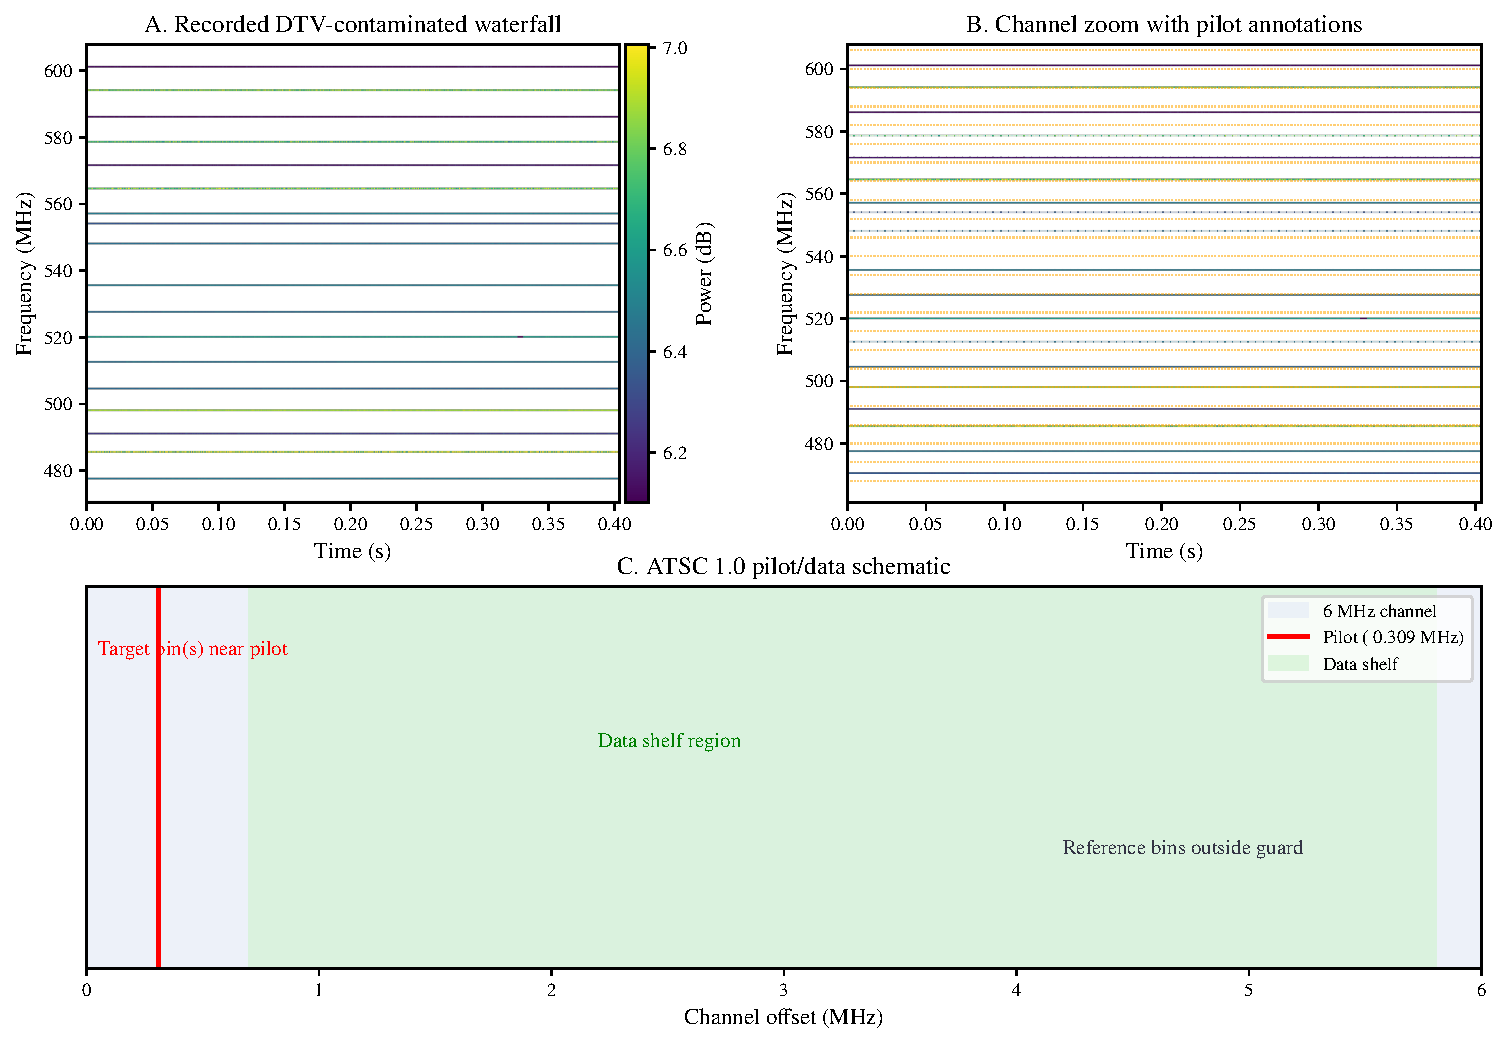
\includegraphics[width=0.95\linewidth]{fig01_dtv_context.pdf}
  \caption{DTV contamination context and ATSC 1.0 pilot structure. Panel A shows a recorded DTV-contaminated waterfall. Panel B gives the channel/pilot context. Panel C sketches the 6 MHz ATSC channel, the pilot near the lower edge, the data shelf, and the target/reference concept used by the detector.}
  \label{fig:context}
\end{figure}

The current recorded-data figure pipeline uses an offline \texttt{spectrogram.npz} cache produced from local recorded data. This is a convenience layer for reproducible plotting and preflight checks. It is not intended to define the production interface. In deployment, detector kernels should operate on individual telescope data streams independently and emit per-stream pilot scores and masks. Those stream-level outputs can then be combined into expanded DTV mask products.

\section{Pilot-tone F-statistic detector}
\label{sec:detector}

The detector compares the local power in target bins around an expected ATSC pilot against reference bins separated from the target by guard bins. The guard bins reduce leakage from the pilot into the reference estimate, while the reference bins estimate the local background level. Figure~\ref{fig:geometry} summarizes the geometry.

Let $\widehat{P}_{\rm target}$ denote the accumulated target-bin power and $\widehat{P}_{\rm reference}$ the accumulated reference-bin power. The detection statistic is
\begin{equation}
  \fstat = \frac{\widehat{P}_{\rm target}}{\widehat{P}_{\rm reference}} .
  \label{eq:fstat}
\end{equation}
Under the null hypothesis $H_0$, the target and reference accumulations are modeled as independent scaled chi-square variables, so that
\begin{equation}
  \fstat \sim F(df_1, df_2) \quad \text{under } H_0.
  \label{eq:null}
\end{equation}
For the detector configuration used in this manuscript,
\begin{equation}
K=128, \quad M=1{,}048{,}576, \quad df_1=2{,}097{,}152, \quad df_2=4{,}194{,}304 .
\end{equation}
The corresponding fine-bin width is \SI{3051.7578125}{Hz}. We use four guard bins, giving a reference offset of \SI{12207.03125}{Hz}. The default operating point used for the real-data demonstration is $\pfa=10^{-3}$, corresponding to $\fstat=1.0037122049331666$.

\begin{figure}[t]
  \centering
  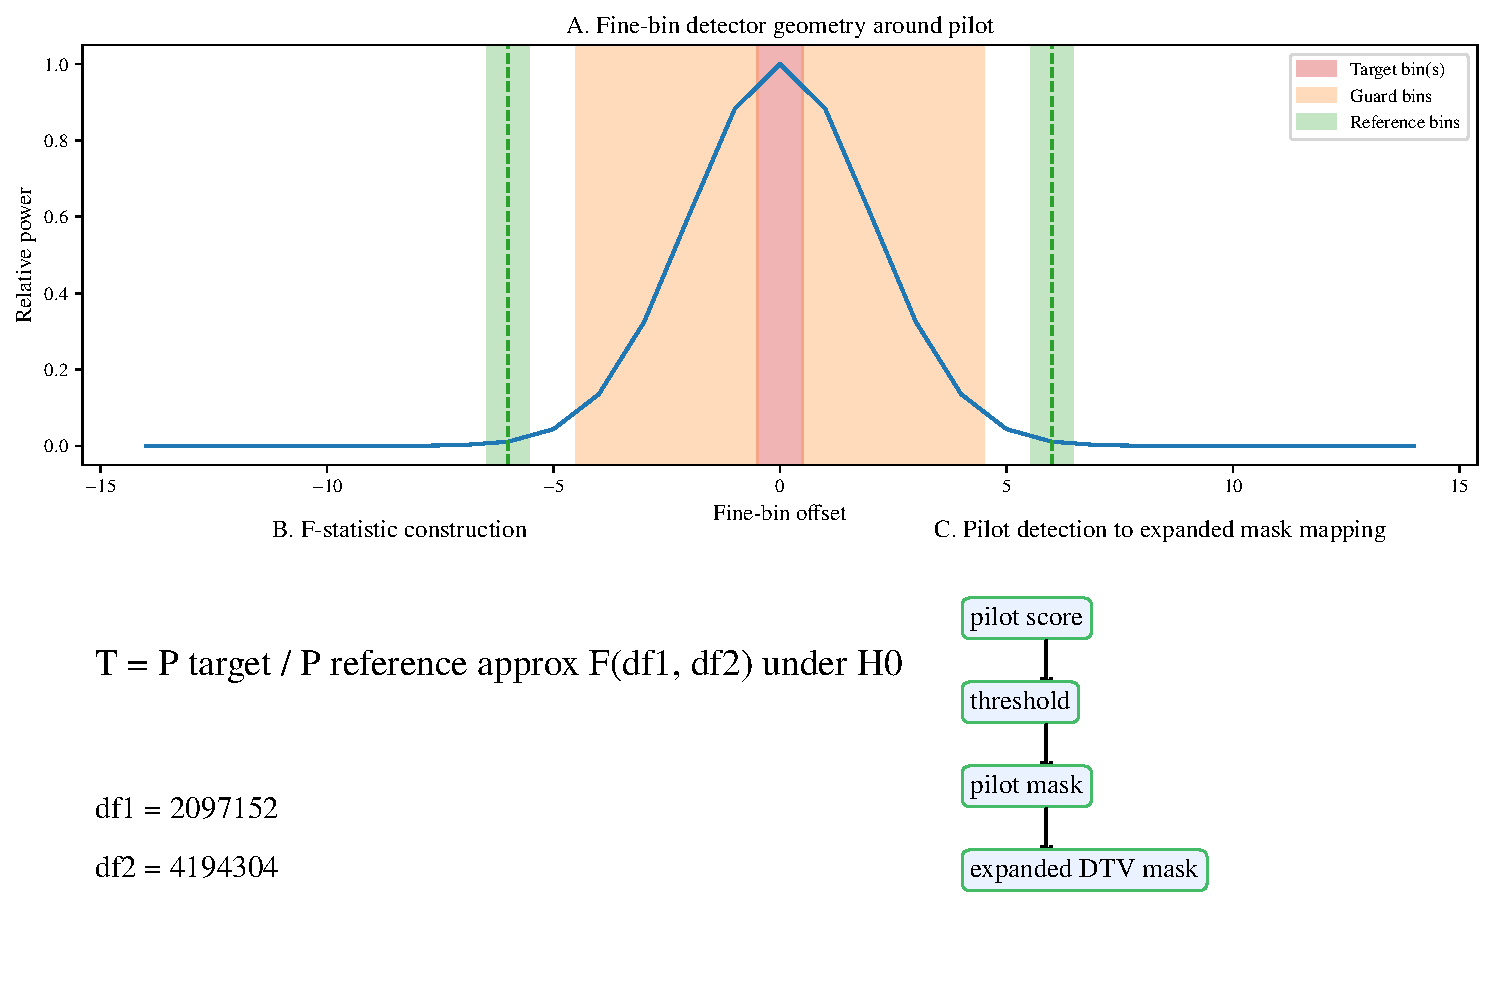
\includegraphics[width=0.95\linewidth]{fig02_detector_geometry.pdf}
  \caption{Detector geometry and F-statistic construction. Panel A shows target, guard, and reference bins around a pilot. Panel B shows the null model for the target/reference ratio. Panel C illustrates the mapping from pilot scores to thresholded pilot masks and expanded DTV masks.}
  \label{fig:geometry}
\end{figure}

The key output of the detector is not only a binary flag, but also a calibrated threshold axis. For any desired false-alarm target $\pfa$, the null model defines a threshold $\eta(\pfa)$ by
\begin{equation}
  \Pr\left(\fstat > \eta(\pfa) \mid H_0\right) = \pfa .
\end{equation}
This constant-false-alarm-rate (CFAR) threshold is useful for detector characterization. Later, science-specific work can map this detector axis to a BAO noise-loss tolerance.

\section{Null calibration and detection sensitivity}
\label{sec:calibration}

\subsection{Null distribution}

Figure~\ref{fig:null_cfar} compares the measured null distribution to the analytic F distribution. The null run used 300,000 Monte Carlo trials. The Kolmogorov-Smirnov statistic was 0.00127 with $p=0.718$, indicating agreement between the simulated null samples and the analytic model at the tested depth. Empirical support is reliable through approximately $\pfa=10^{-4}$; below $3.33\times10^{-5}$, fewer than ten expected tail samples are available and the plotted tail is theory/model-supported.

\begin{figure}[t]
  \centering
  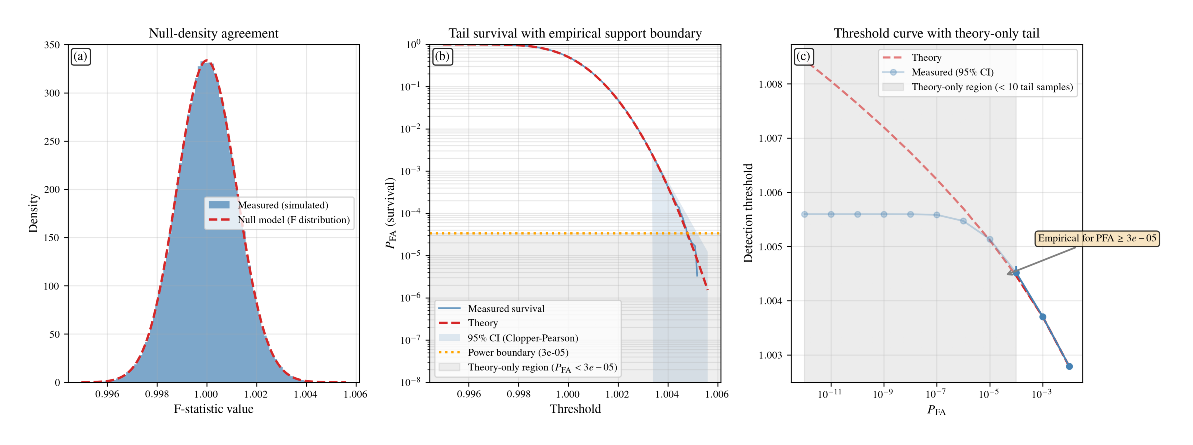
\includegraphics[width=0.95\linewidth]{fig03_null_cfar_validation.pdf}
  \caption{Null-distribution and CFAR calibration for the K=128 detector. Panel A compares the simulated null density to the F-distribution model. Panel B shows the survival function with confidence intervals and empirical support boundary. Panel C shows the threshold curve; the shaded region marks false-alarm rates with fewer than ten expected tail samples in the null simulation.}
  \label{fig:null_cfar}
\end{figure}

\subsection{Sensitivity calibration}

Figure~\ref{fig:sensitivity} reports the required DTV data-shelf SNR as a function of target false-alarm probability and target detection probability. The empirical points use 12,000 injection trials and binomial confidence intervals. The figure also includes an empirical detection-probability map $\widehat{P}_D(\mathrm{SNR},\pfa)$.

\begin{figure}[t]
  \centering
  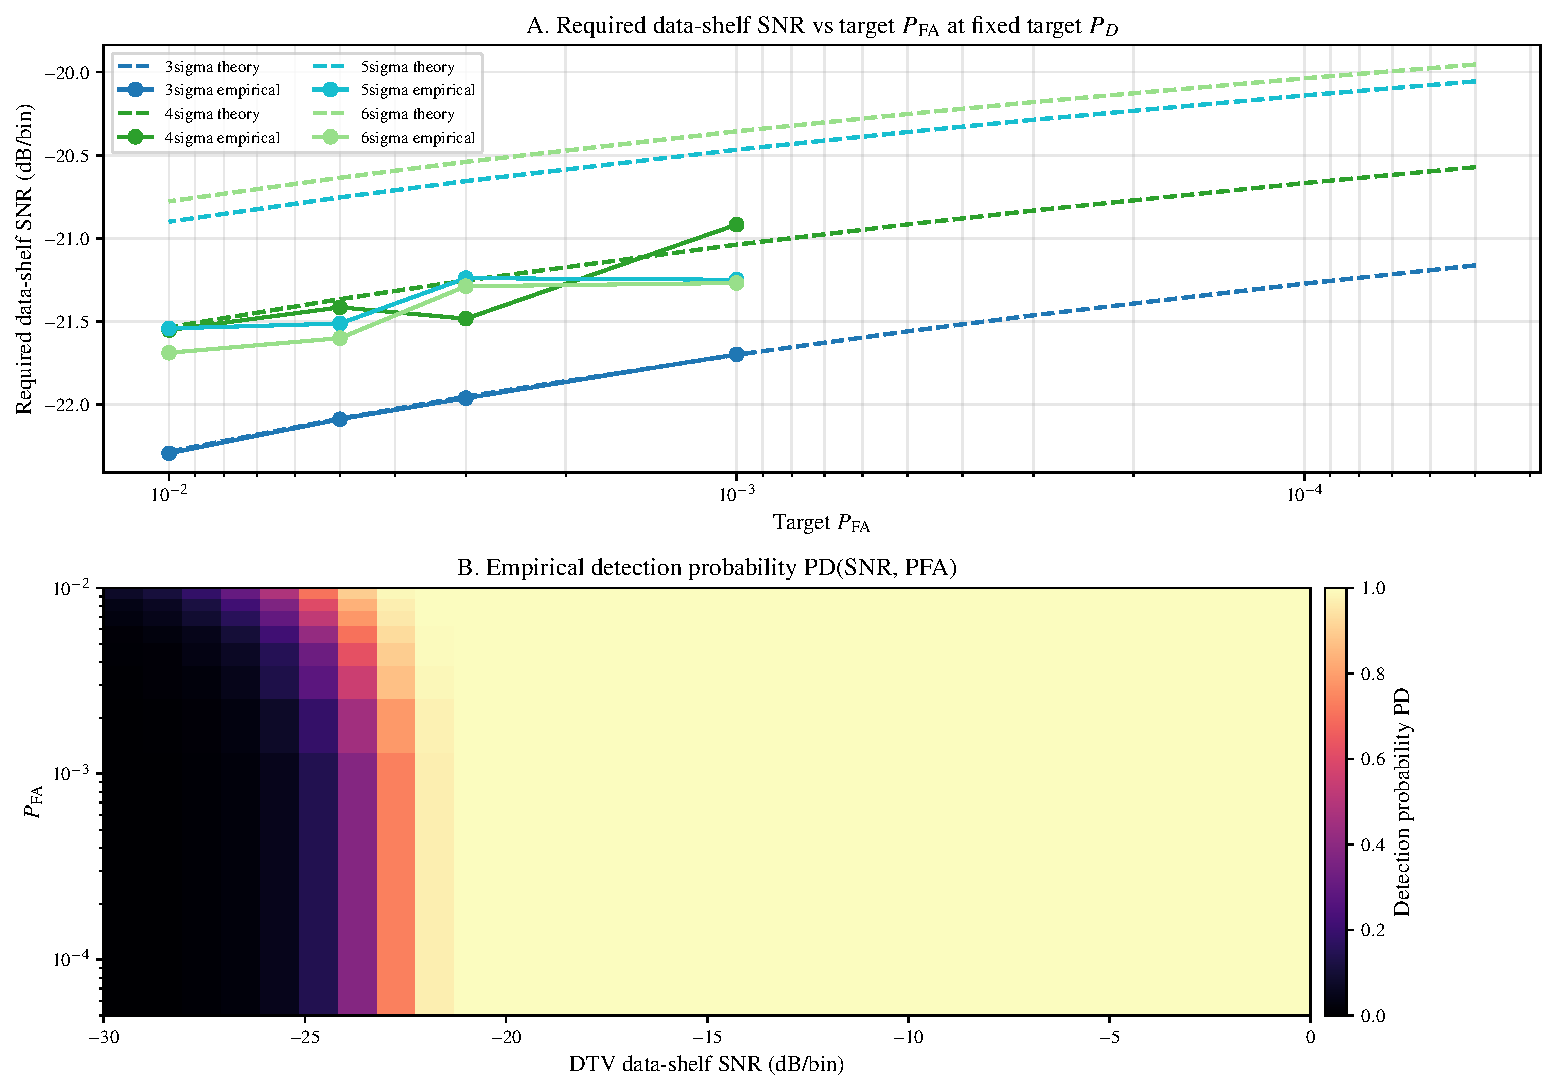
\includegraphics[width=0.95\linewidth]{fig04_detection_sensitivity_k128.pdf}
  \caption{Detection sensitivity for the K=128, guard=4 detector. Panel A shows the required DTV data-shelf SNR for several target detection probabilities as a function of target false-alarm probability. Panel B shows empirical detection probability as a function of data-shelf SNR and $\pfa$. Extreme high-$P_D$ and low-tail-support points are model-supported and should be interpreted with the finite-trial caveat described in the text.}
  \label{fig:sensitivity}
\end{figure}

The finite-trial caveat matters most at the largest target detection probabilities and smallest false-alarm probabilities. For example, a false-alarm target of $5\times10^{-5}$ corresponds to fewer than one expected false alarm in the 12,000 injection trials used for the sensitivity sweep. We therefore treat the empirical values as consistency checks on the analytic/model-supported detector axis rather than as independent validation of arbitrarily deep tails.

\section{Robustness and design choices}
\label{sec:robustness}

The detector should be stable against practical deviations from the idealized pilot location and noise model. Figure~\ref{fig:robustness} summarizes the current robustness tests. Within-bin offsets produce increasing detection loss as the pilot approaches a half-bin displacement. The worst half-bin structured loss is approximately 3.52 dB, while the average random within-bin loss is approximately 1.43 dB. The current pass criterion is 4.25 dB, so the half-bin case remains within the design tolerance. Doppler offsets and gain/noise perturbations remain bounded over the tested range. Guard-bin leakage tests select four guard bins, consistent with the current detector build.

\begin{figure}[t]
  \centering
  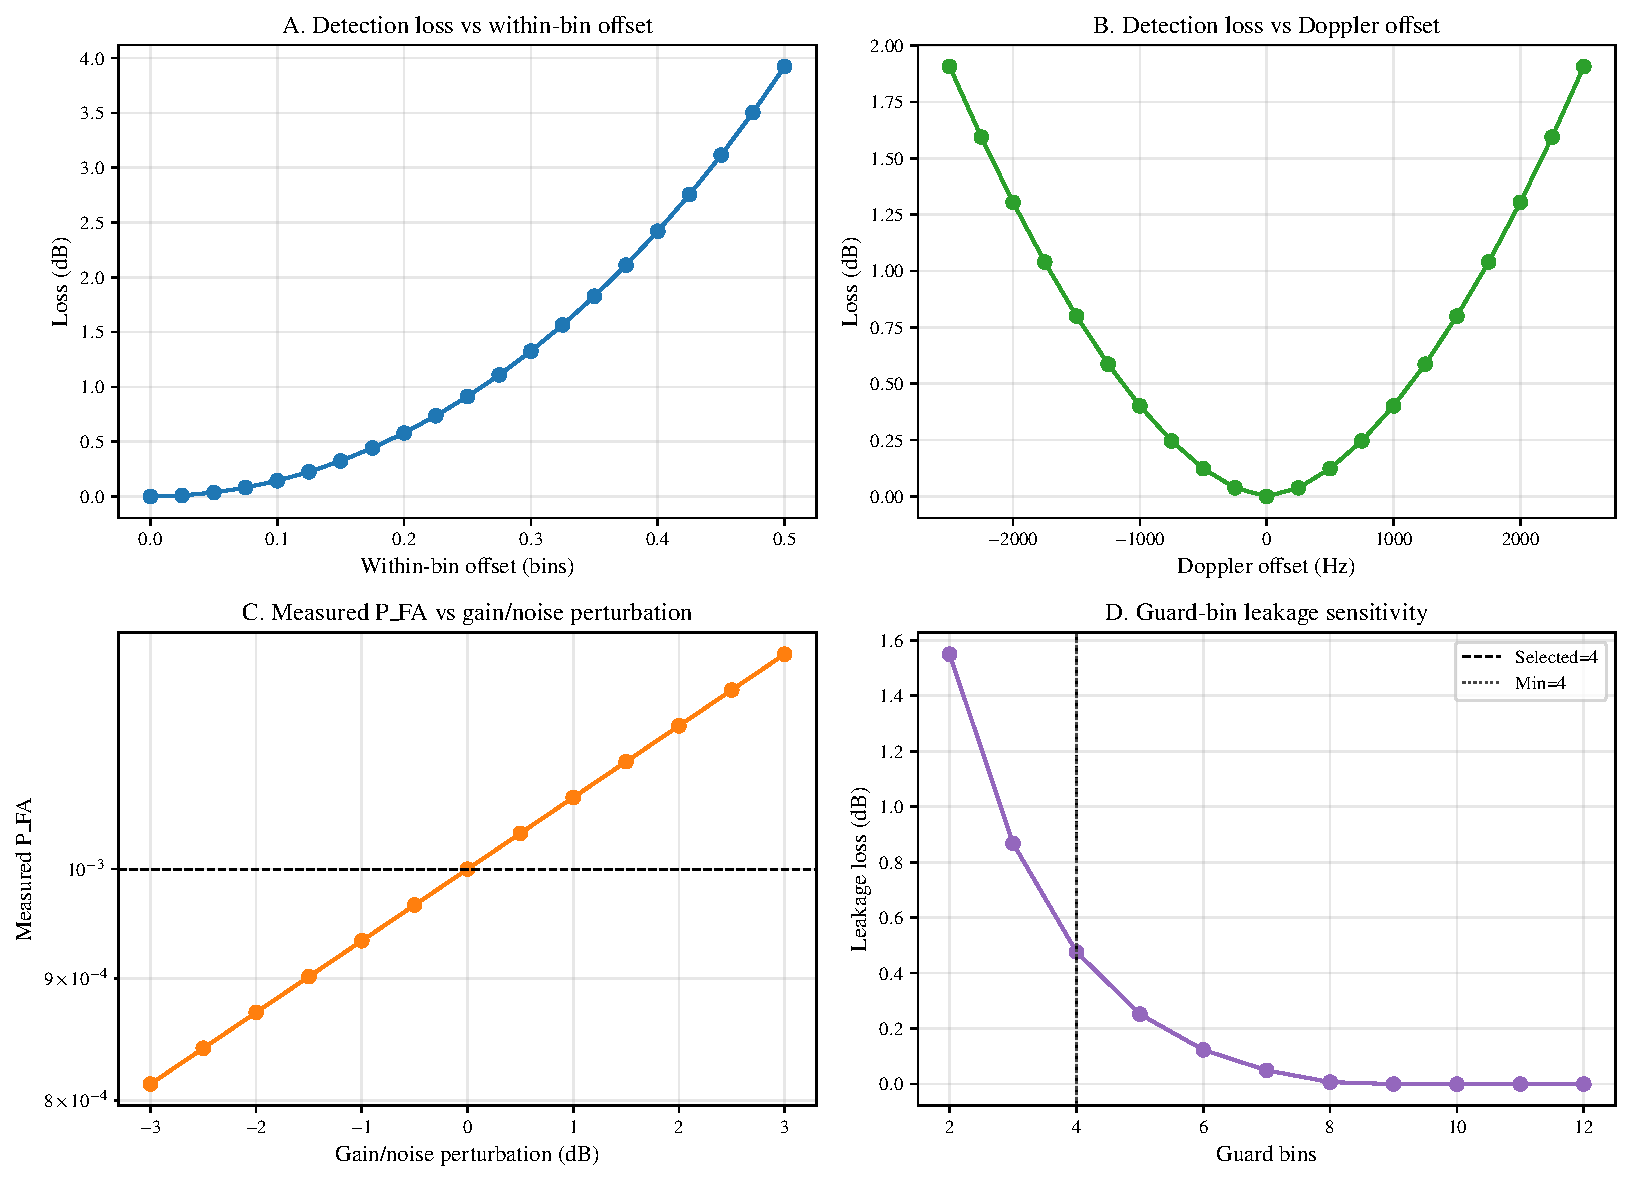
\includegraphics[width=0.95\linewidth]{fig05_robustness_summary.pdf}
  \caption{Robustness summary. Panel A shows detection loss versus within-bin offset. Panel B shows Doppler-offset loss. Panel C shows measured false-alarm behavior under gain/noise perturbations. Panel D shows leakage loss versus guard-bin selection; the selected and minimum guard counts are both four bins.}
  \label{fig:robustness}
\end{figure}

The guard-bin test is particularly important because the reference estimate must remain local enough to track the background but far enough away from the pilot to avoid leakage. The present design uses the minimum guard count satisfying the leakage-loss criterion. 

\section{Fixed-point GPU prototype}
\label{sec:implementation}

A production detector must be compatible with the telescope data stream and must be efficient enough for real-time or near-real-time operation. Figure~\ref{fig:kernel} summarizes the current prototype implementation. The pipeline accumulates input spectra, computes target and reference powers, forms the F-statistic, thresholds the scores, and emits mask products. The figure also compares fixed-point outputs with a floating-point reference and shows the current throughput benchmark.

\begin{figure}[t]
  \centering
  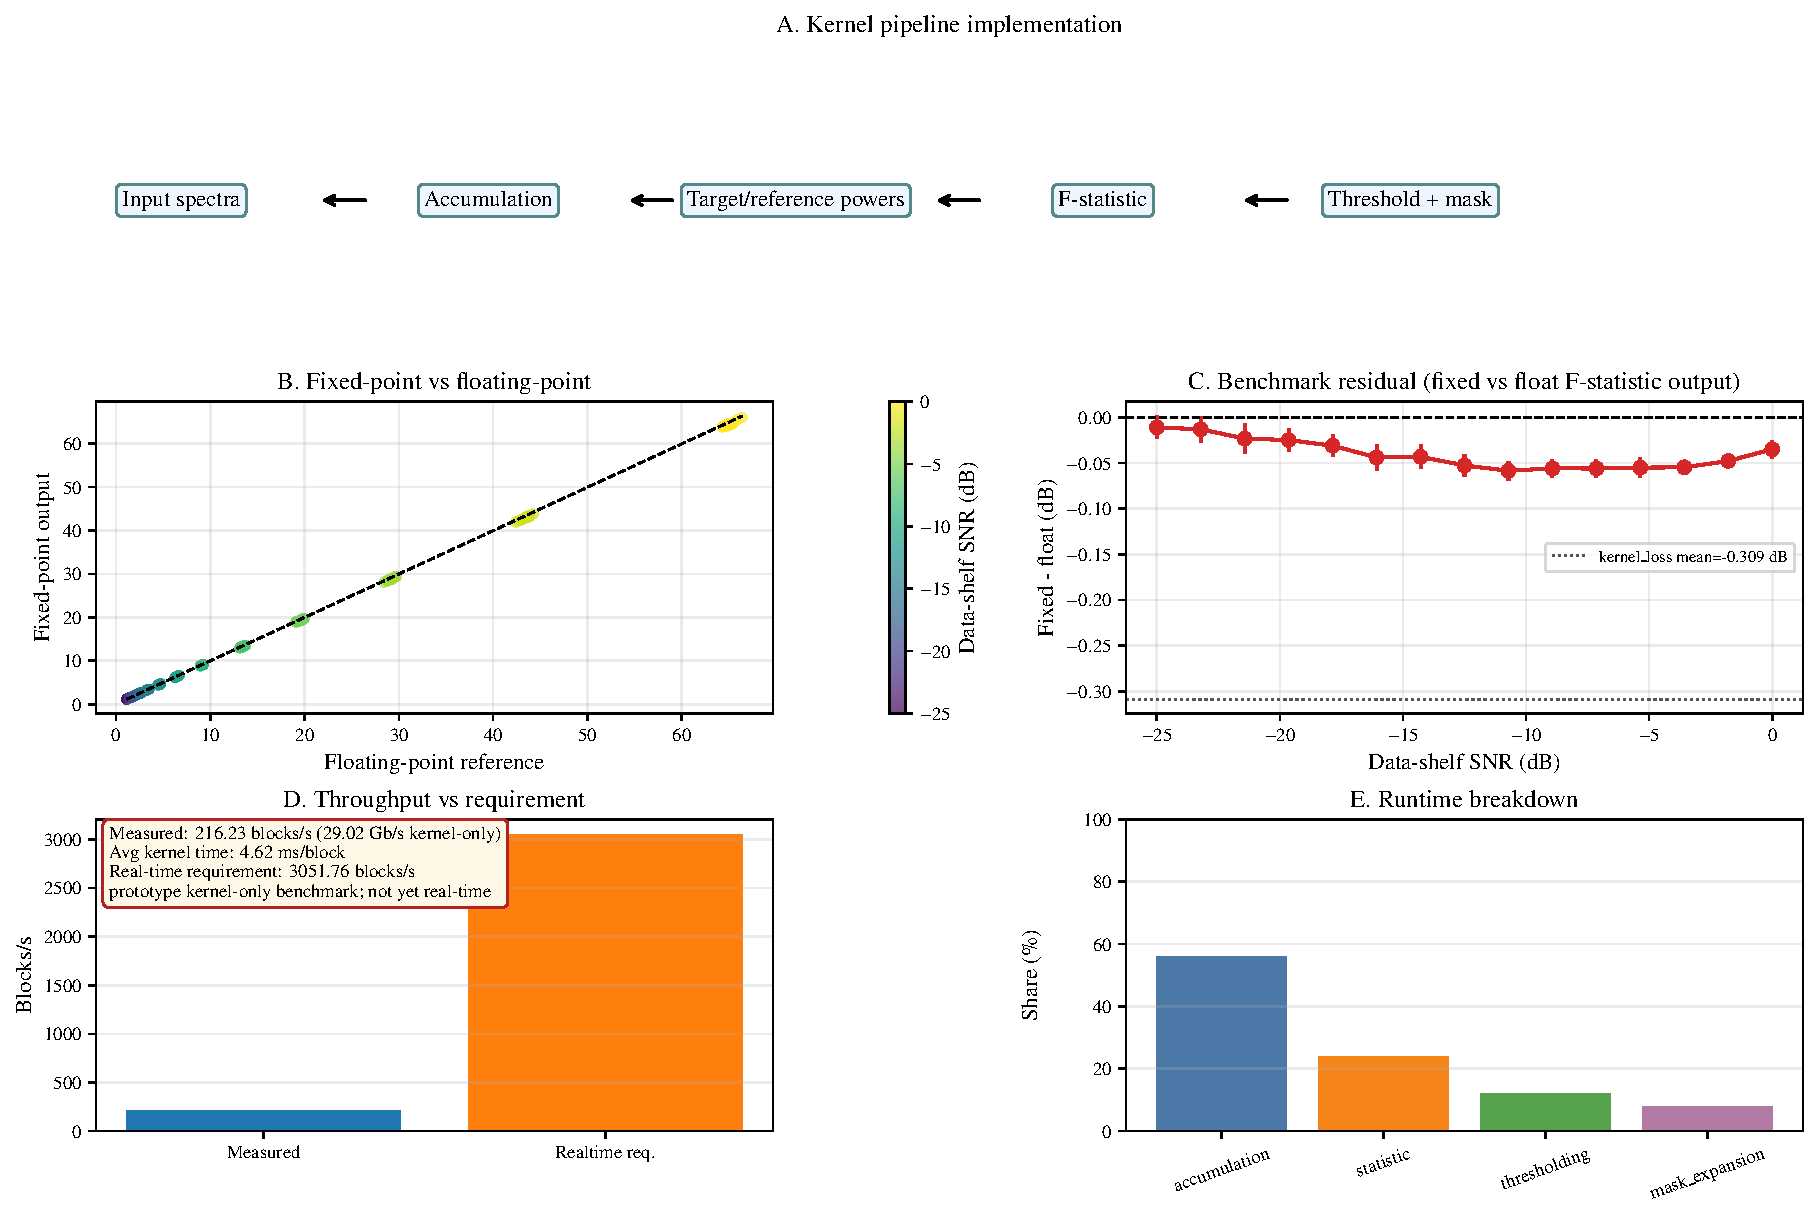
\includegraphics[width=0.95\linewidth]{fig06_kernel_implementation.pdf}
  \caption{Kernel implementation characterization. Panel A shows the detector-kernel pipeline. Panel B compares fixed-point and floating-point outputs. Panel C shows the residual implementation bias. Panel D compares measured kernel throughput to the real-time block-rate requirement. Panel E shows the runtime breakdown. The benchmark is kernel-only and excludes host/device transfers. The current prototype is not yet real-time.}
  \label{fig:kernel}
\end{figure}

The latest rendered benchmark shows a kernel-only throughput of 216.23 blocks/s, or 29.02 Gb/s, with an average kernel time of 4.62 ms/block. The real-time requirement for the current block definition is 3051.76 blocks/s. The prototype is therefore approximately a factor of 14 below the current block-rate requirement. This should be interpreted as an implementation characterization and optimization target, not as a completed production deployment.

The fixed-point characterization indicates a mean implementation bias of approximately $-0.309$ dB over the validated data-shelf SNR range, with maximum absolute bias of approximately 0.59 dB. These values are acceptable for detector characterization, but production deployment will require further optimization, pipeline integration, and validation against live-stream constraints.

\section{Recorded-data demonstration}
\label{sec:realdata}

Figure~\ref{fig:realdata} shows a single recorded DTV-contaminated segment processed by the K=128 detector. The panels show the raw waterfall, pilot score map, pilot-level binary detection mask, expanded DTV mask, and overall masked fraction versus block index. The operating point is $\pfa=10^{-3}$ with $\eta=1.0037122049331666$.

\begin{figure}[t]
  \centering
  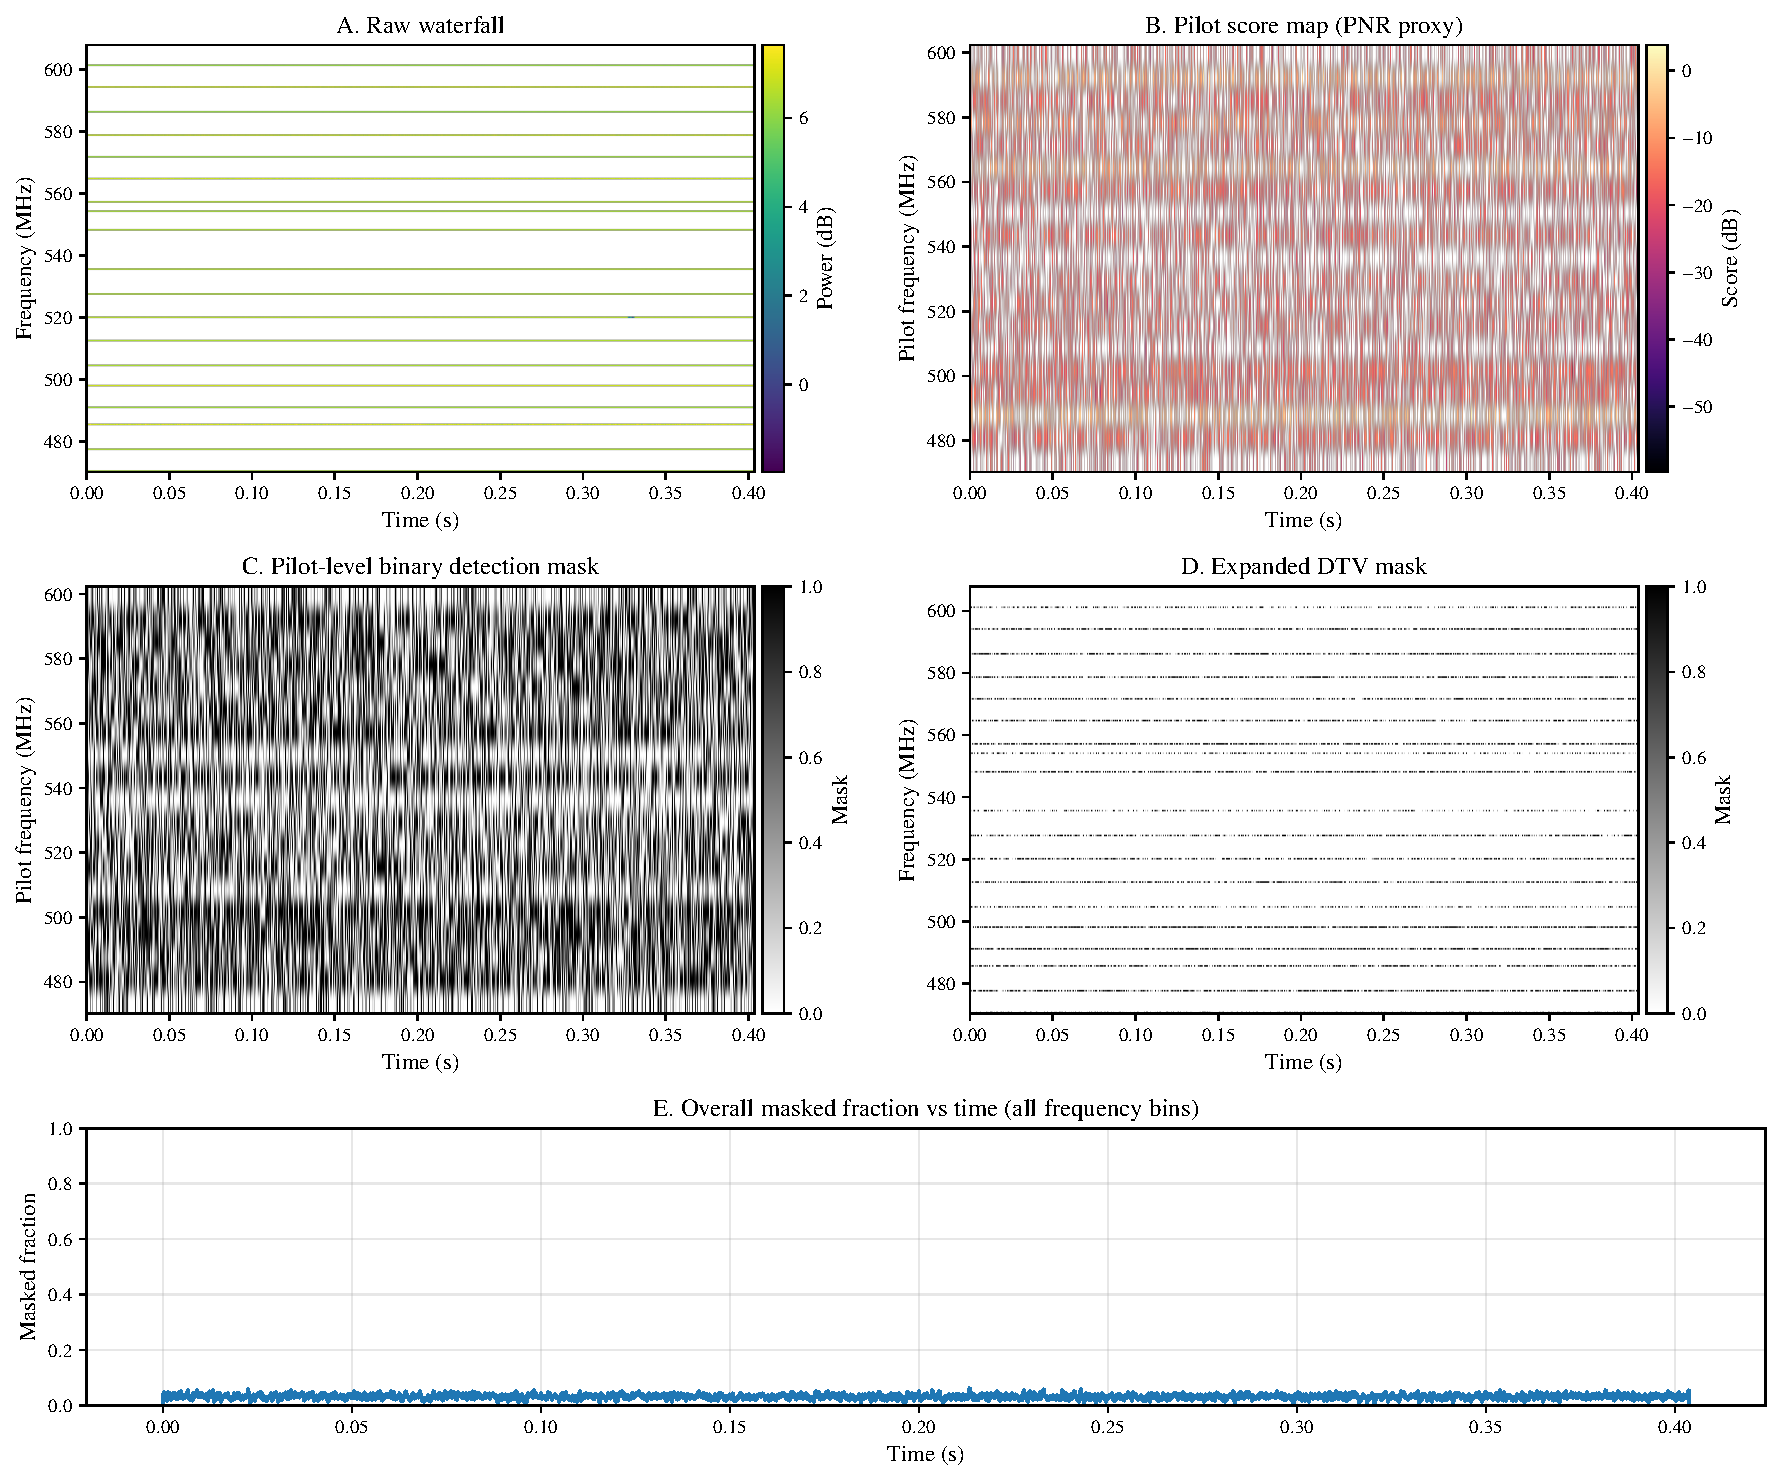
\includegraphics[width=0.95\linewidth]{fig07_realdata_score_and_mask.pdf}
  \caption{Single-segment recorded-data demonstration. Panel A shows the raw waterfall. Panel B shows the pilot score map, using a PNR proxy based on $10\log_{10}(\max(T-1,0))$. Panel C shows the pilot-level binary detection mask. Panel D shows the expanded DTV mask. Panel E shows the overall masked fraction versus block index. This is not archive-scale validation.}
  \label{fig:realdata}
\end{figure}

This example demonstrates that the detector produces a structured mask on recorded data and that detections occur at plausible DTV pilot locations. It should not be interpreted as a statistical survey of telescope performance. The processed duration is only 0.404 s, so it does not probe day-to-day propagation changes, independent observing windows, or low/representative/high RFI regimes.

\section{Deferred validation and planned additions}
\label{sec:todos}

This draft intentionally separates the detector/implementation contribution from the remaining validation tasks. The following items should be completed before final journal submission or moved explicitly to future work.

\subsection{Matched finite-sample baseline comparison}

Possible baselines include an energy detector applied to the target bins and a local shelf-power threshold. The comparison must use the same injected signal convention and the same false-alarm calibration as the F-statistic detector. Otherwise, the comparison will be visually compelling but statistically misleading.

\subsection{Archive-scale validation}

The final validation section should report, at minimum, the distribution of mask burden, active pilot count, residual pilot score, retained fraction, and failure cases across candidate windows. This will convert the single-segment demonstration into a telescope-relevant operational validation.

\subsection{Science-driven threshold selection}

The threshold in this paper is CFAR-calibrated. That is appropriate for detector characterization, but the final operational threshold should be science-driven. For BAO science, a natural next step is to perturb the noise covariance in a Fisher forecast and determine the excess-noise level that produces an acceptable degradation in $D_V(z)$ or related BAO observables \cite{Bull2015,RadioFisher2021}. The detector threshold can then be selected by mapping detector score, mask burden, and residual contamination to that tolerance.

\subsection{Production stream interface}

The offline \texttt{spectrogram.npz} cache is useful for figures, but production operation should process independent HDF5 or live telescope streams. The deployed kernel should operate on each stream separately, emit per-stream pilot scores, and then pass those outputs to a later mask-expansion stage.

\section{Discussion}
\label{sec:discussion}

The results support the detector as a calibrated instrumentation method. The null model is accurate over the supported Monte Carlo depth, the threshold axis is explicit, and the sensitivity curves show the detector operating in the weak-DTV regime. The robustness tests indicate that the selected K=128, guard=4 geometry is a reasonable working point. The GPU prototype demonstrates that the computation is implementable in a fixed-point kernel, although the current benchmark remains below the real-time block-rate requirement.

The principal limitation is the lack of archive-scale recorded-data validation in the present draft. This is a deliberate scope decision. The current paper establishes the detector, calibration, robustness, implementation, and a recorded-data demonstration. The long-duration deployment study should be a separate telescope-integration result or an expanded final version of this paper once data are available.

The second limitation is threshold interpretation. A CFAR threshold is statistically clean, but it does not directly encode the downstream cost of masking too much data or leaving residual RFI. This paper therefore treats $\pfa=10^{-3}$ as a representative operating point, not as the final science threshold. The final threshold should be selected using a science-loss tolerance, especially for 21 cm BAO analyses.

\section{Conclusions}
\label{sec:conclusion}

We have developed a pilot-tone F-statistic detector for ATSC 1.0 DTV interference in radio astronomy data streams. The detector uses target, guard, and reference bins around the known pilot location and is calibrated by an analytic F-distributed null model. For the K=128, guard=4 configuration, the null calibration agrees with simulation through the supported tail depth, and the detector provides a controllable CFAR threshold axis. Sensitivity and robustness tests characterize detection performance under within-bin offset, Doppler offset, gain/noise perturbation, and reference-bin leakage. A fixed-point CUDA prototype reproduces the floating-point reference within the validated bias range, although the current kernel-only benchmark remains below real-time throughput. A single recorded-data segment demonstrates pilot-level and expanded DTV mask generation.

The next steps are archive-scale validation, matched finite-sample baseline comparison, and science-driven threshold selection. These additions will determine the final operational threshold and quantify telescope-scale performance across realistic RFI conditions.

\section*{Acknowledgments}
-

\section*{Code, data, and reproducibility}
-

\printbibliography

\end{document}
